\documentclass{article}
\topmargin -0.5in \oddsidemargin -0.25in \textheight 9in
\textwidth 6.5in
\usepackage{graphics}
\usepackage{graphicx}
\usepackage{forest}
\usepackage{tikz}
\usepackage{amsmath}
\usepackage{amssymb}
\usepackage{multirow}
\usepackage{siunitx}

\begin{document}
{\bf ICS 271}

{\bf Fall 2016}

{\bf Student ID : 26642334}

{\bf Student Name: Yu Guo}

{\bf Instructor : Kalev Kask}

{\bf Homework Assignment 4}

{\bf Due Thursday, 11/3}




\begin{enumerate}

% 1.
\item

$X = \{v_1,v_2,v_3,v_4,v_5,v_6\}$ \\ \\
$D = \{D_1,D_2,D_3,D_4,D_5,D_6\}$ \\
- $D_1 = $ \{desk, easy, dove, else, help, kind, soon, this\} \\
- $D_2 = $ \{eta, hat, her, him, one\} \\
- $D_3 = $ \{at, be, he, it, on\} \\
- $D_4 = $ \{dance, usage, first, loses, fuels, haste, given, sense, sound, think\} \\
- $D_5 = $ \{dance, usage, first, loses, fuels, haste, given, sense, sound, think\} \\
- $D_6 = $ \{desk, easy, dove, else, help, kind, soon, this\} \\ \\
$C_1 = \{v_2(1)=v_1(2), v_2(2)=v_3(2), v_2(3)=v_4(3), v_5(1)=v_4(4), v_5(3)=v_6(3)\}$, $v_i(j)$ means the $j$-th letter in word $i$. \\
$C_2 = \{v_1 \neq v_6, v_4 \neq v_5\}$ \\ \\
Cost function: the number of constraints unsatisified. (Range from 0 to 5) \\ \\
Start: $v_1$=this, $v_2$=eta, $v_3$=at, $v_4$=dance, $v_5$=haste, $v_6$=dove, cost=4\\
Iter1: $v_1$=help, $v_2$=eta, $v_3$=at, $v_4$=dance, $v_5$=haste, $v_6$=dove, cost=3, update $v_1$\\
Iter2: $v_1$=help, $v_2$=eta, $v_3$=at, $v_4$=usage, $v_5$=haste, $v_6$=dove, cost=2, update $v_4$\\
Iter3: $v_1$=help, $v_2$=eta, $v_3$=at, $v_4$=usage, $v_5$=given, $v_6$=dove, cost=0, update $v_5$\\


% 2.
\item
Assume there's a classes(subjects) list $S$, the number of elements in $S$ is $NoS$, $s_i$ is $i$-th subject in $S$, $i=1,2,\dots,NoS$. We have, \\
$$ S = \{s_i, i=1,2,\dots,NoS\} $$ \\
Same as professors($P$), classesrooms($C$) and timeslots($T$). That we have,
$$ P = \{p_\alpha, \alpha=1,2,\dots,NoP\} $$ 
$$ C = \{c_\beta, \beta=1,2,\dots,NoC\} $$ 
$$ T = \{t_\gamma, \gamma=1,2,\dots,NoT\} $$ 

$X = \{ (s_i, p_\alpha, c_\beta, t_\gamma), i=1,2,\dots,NoS\}$, it means that subject $s_i$ is taught by professor $p_\alpha$ at classroom $c_\beta$ on timeslot $t_\gamma$. \\ \\
$D_j = \{ (s_i, p_\alpha, c_\beta, t_\gamma) | i,\alpha,\beta,\gamma$ could be any valid value\} \\ \\
$C$: - Each $s_i$ should only appear once. \\
- For any two subjects $(s_{i1}, p_{\alpha1}, c_{\beta1}, t_{\gamma1})$ and $(s_{i2}, p_{\alpha2}, c_{\beta2}, t_{\gamma2})$, \\
if $p_{\alpha1}=p_{\alpha2}$, then $t_{\gamma1} \neq t_{\gamma2}$, it means a professor could not have two classes at same time; \\
if $c_{\beta1}=c_{\beta2}$, then $t_{\gamma1} \neq t_{\gamma2}$, it means one classroom could no have two classes at same time.

% 3.
\item
Assume big rectangle locate in a 2-$D$ coordinate system, range from $[0,X]\times[0,Y]$. \\ \\
$X = \{(x_i,y_i,dX_i,dY_i) | i=1,2,\dots,n\}$, each $X_i$ represents a small rectangle with it's position(bottom left corner) ($x_i,y_i$) and size ($dX_i,dY_i$). \\ \\
$D_i = \{(x,y,dX,dY) | dX \leqslant X, dY \leqslant Y\}$ \\ \\
$C_1$: For each small rectangle $(x_i,y_i,dX_i,dY_i)$, we have, \\
$ x_i \geqslant 0 $ and 
$ x_i+dX \leqslant X $ and
$ y_i \geqslant 0 $ and 
$ y_i+dY \leqslant Y $

$C_2$: For any of two small rectangles $(x_i,y_i,dX_i,dY_i)$ and $(x_j,y_j,dX_j,dY_j)$, we have, \\
$ x_i + dX_i \leqslant x_j $ or 
$ x_j + dX_j \leqslant x_i $ or 
$ y_i + dY_i \leqslant y_j $ or 
$ y_j + dY_j \leqslant y_i $





% 4.
\item
    \begin{enumerate}
    \item
    For any neighboring pair of squares $i$ and $j$ such that $i \neq j$, \\
    % Relation: $|X_i-X_j| \geqslant 2$ \\
    % Domain: (1,3), (1,4), (1,5), (1,6), (1,7), (1,8), (1,9), \\
    %         (2,4), (2,5), (2,6), (2,7), (2,8), (2,9), \\
    %         (3,1), (3,5), (3,6), (3,7), (3,8), (3,9), \\
    %         (4,1), (4,2), (4,6), (4,7), (4,8), (4,9), \\
    %         (5,1), (5,2), (5,3), (5,7), (5,8), (5,9), \\
    %         (6,1), (6,2), (6,3), (6,4), (6,8), (3,9), \\
    %         (7,1), (7,2), (7,3), (7,4), (7,5), (7,9), \\
    %         (8,1), (8,2), (8,3), (8,4), (8,5), (8,6), \\
    %         (9,1), (9,2), (9,3), (9,4), (9,5), (9,6), (9,7)

    \begin{table}[h]
    \centering
    \begin{tabular}{|c|c|}
    \hline
    Relation & Domain \\
    \hline
    \multirow{9}{*}{$|X_i-X_j| \geqslant 2$} & (1,3), (1,4), (1,5), (1,6), (1,7), (1,8), (1,9), \\
            & (2,4), (2,5), (2,6), (2,7), (2,8), (2,9), \\
            & (3,1), (3,5), (3,6), (3,7), (3,8), (3,9), \\
            & (4,1), (4,2), (4,6), (4,7), (4,8), (4,9), \\
            & (5,1), (5,2), (5,3), (5,7), (5,8), (5,9), \\
            & (6,1), (6,2), (6,3), (6,4), (6,8), (3,9), \\
            & (7,1), (7,2), (7,3), (7,4), (7,5), (7,9), \\
            & (8,1), (8,2), (8,3), (8,4), (8,5), (8,6), \\
            & (9,1), (9,2), (9,3), (9,4), (9,5), (9,6), (9,7) \\
    \hline      
    \end{tabular}
    \end{table}

    \begin{center}
    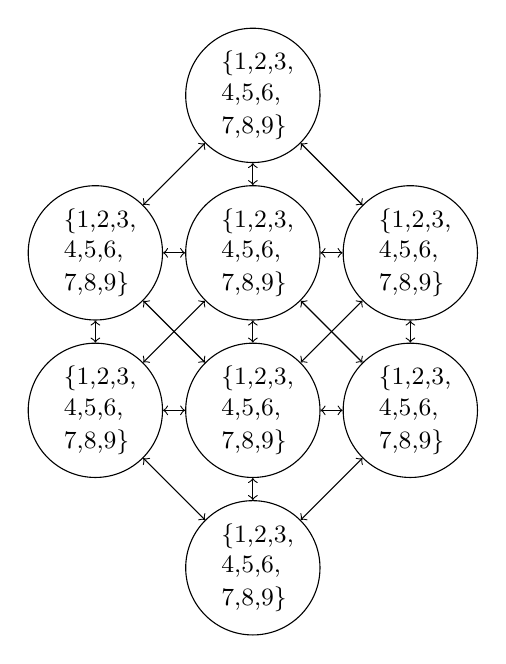
\begin{tikzpicture}
      \node[circle,draw] (1) at ( 0, 0) [text width=0.8cm] {\small \{1,2,3,\\4,5,6,\\7,8,9\}};
      \node[circle,draw] (2) at (-2,-2) [text width=0.8cm] {\small \{1,2,3,\\4,5,6,\\7,8,9\}};
      \node[circle,draw] (3) at ( 0,-2) [text width=0.8cm] {\small \{1,2,3,\\4,5,6,\\7,8,9\}};
      \node[circle,draw] (4) at ( 2,-2) [text width=0.8cm] {\small \{1,2,3,\\4,5,6,\\7,8,9\}};
      \node[circle,draw] (5) at (-2,-4) [text width=0.8cm] {\small \{1,2,3,\\4,5,6,\\7,8,9\}};
      \node[circle,draw] (6) at ( 0,-4) [text width=0.8cm] {\small \{1,2,3,\\4,5,6,\\7,8,9\}};
      \node[circle,draw] (7) at ( 2,-4) [text width=0.8cm] {\small \{1,2,3,\\4,5,6,\\7,8,9\}};
      \node[circle,draw] (8) at ( 0,-6) [text width=0.8cm] {\small \{1,2,3,\\4,5,6,\\7,8,9\}};
 
      \path[<->] (1) edge (2);
      \path[<->] (1) edge (3);
      \path[<->] (1) edge (4);
      \path[<->] (2) edge (3);
      \path[<->] (3) edge (4);
      \path[<->] (2) edge (5);
      \path[<->] (2) edge (6);
      \path[<->] (3) edge (5);
      \path[<->] (3) edge (6);
      \path[<->] (3) edge (7);
      \path[<->] (4) edge (6);
      \path[<->] (4) edge (7);
      \path[<->] (5) edge (6);
      \path[<->] (6) edge (7);
      \path[<->] (5) edge (8);
      \path[<->] (6) edge (8);
      \path[<->] (7) edge (8);
    \end{tikzpicture}
    \end{center}


    \item
    Yes, it's arc-consistent.
    
    \item
    Yes, it's consistent. One solution is,

    \begin{table}[h]
    \centering
    \begin{tabular}{l|l|l}
    \cline{2-2}
                            & 2 &                        \\ \hline
    \multicolumn{1}{|l|}{5} & 8 & \multicolumn{1}{l|}{6} \\ \hline
    \multicolumn{1}{|l|}{3} & 1 & \multicolumn{1}{l|}{4} \\ \hline
                            & 7 &                        \\ \cline{2-2}
    \end{tabular}
    \end{table}

    \end{enumerate}

% 5.
\item
    \begin{enumerate}
    \item
    Yes, it's arc-consistent.
    
    \begin{center}
    \begin{forest}
    for tree={ellipse,draw,edge=-}
    [{7,8}
        [{5,6}
            [{3,4}
                [{1,2}]
                [{1,2}]
            ]
            [{3,4}
                [{1,2}]
                [{1,2}]
            ]
        ]
        [{5,6}
            [{3,4}
                [{1,2}]
                [{1,2}]
            ]
            [{3,4}
                [{1,2}]
                [{1,2}]
            ]
        ]
    ]
    \end{forest}
    \end{center}

    \item
    Yes, it's consistent. One solution is,
    $$ X_1 = 8 ~~ X_2 = 6 ~~ X_3 = 6 $$
    $$ X_4 = 4 ~~ X_5 = 4 ~~ X_6 = 4 ~~ X_7 = 4 $$
    $$ X_8 = 2 ~~ X_9 = 2 ~~ X_{10} = 2 ~~ X_{11} = 2 $$
    $$ X_{12} = 2 ~~ X_{13} = 2 ~~ X_{14} = 2 ~~ X_{15} = 2 $$

    \item
    Do an in-order traversal: 1, 2, 3, 4, 5, 6, 7, 8, 9, 10, 11, 12, 13, 14, 15

    \item
    Since this is a tree the complexity is $O(nd^2)$ when $n$ is the number of variables and $d$ is the domain size.
    \end{enumerate}

% 6.
\item
Solve problem:
\begin{table}[h]
\centering
\begin{tabular}{lllll}
  &   & T & W & O \\
+ &   & T & W & O \\ \hline
  & F & O & U & R
\end{tabular}
\end{table}

Constraints:
$$ O + O = R + 10X_1 $$
$$ W + W + C_1 = U + 10C_2 $$
$$ T + T + C_2 = O + 10C_3 $$
$$ C_3 = F $$
$$ alldiff(T,W,O,F,U,R) $$

Domain:
$$ D_F,D_{C_3} = \{1\} $$
$$ D_{C_1},D_{C_2} = \{0,1\} $$
$$ D_T = \{1,2,3,4,5,6,7,8,9\} $$
$$ D_W,D_O,D_U,D_R = \{0,1,2,3,4,5,6,7,8,9\} $$

A solution: 
\begin{table}[ht]
\centering
\begin{tabular}{lllll}
  &   & 7 & 3 & 4 \\
+ &   & 7 & 3 & 4 \\ \hline
  & 1 & 4 & 6 & 8
\end{tabular}
\end{table}

A trace to a solution:
\begin{table}[ht]
\centering
\begin{tabular}{|m{0.05\linewidth}<{\centering}|m{0.7\linewidth}<{\centering}|m{0.25\linewidth}|}
\hline
Node & State & Action \\
\hline
0 & 
$ D_F,D_{C_3} = \{1\} $,
$ D_{C_1},D_{C_2} = \{0,1\} $,
$ D_T = \{1,2,3,4,5,6,7,8,9\} $,
$ D_W,D_O,D_U,D_R = \{0,1,2,3,4,5,6,7,8,9\} $
& Initial State \\
\hline  
1 & 
$ F=1,D_{C_3}=\{1\} $,
$ D_{C_1},D_{C_2} = \{0,1\} $,
$ D_T = \{2,3,4,5,6,7,8,9\} $,
$ D_W,D_O,D_U,D_R = \{0,2,3,4,5,6,7,8,9\} $
& Assign $F=1$ \\
\hline  
2 & 
$ F=1,C_3=1 $,
$ D_{C_1},D_{C_2} = \{0,1\} $,
$ D_T = \{5,6,7,8,9\} $,
$ D_W,D_O,D_U,D_R = \{0,2,3,4,5,6,7,8,9\} $
& Assign $C_3=1$ \\
\hline
3 & 
$ F=1,C_3=1,C_2=0 $,
$ D_{C_1} = \{0,1\} $,
$ D_T = \{5,6,7,8,9\} $,
$ D_W = \{0,2,3,4\} $,
$ D_O = \{0,2,4,6,8\} $,
$ D_U,D_R = \{0,2,3,4,5,6,7,8,9\} $
& Assign $C_2=0$ \\
\hline     
4 & 
$ F=1,C_3=1,C_2=0,C_1=0 $,
$ D_T = \{5,6,7,8,9\} $,
$ D_W = \{0,2,3,4\} $,
$ D_O = \{0,2,4\} $,
$ D_U = \{0,2,4,6,8\} $
$ D_R = \{0,2,3,4,5,6,7,8,9\} $
& Assign $C_1=0$ \\
\hline      
5 & 
$ F=1,C_3=1,C_2=0,C_1=0, T=6,O=2,R=4 $,
$ D_W = \{0,3\} $,
$ D_U = \{0,8\} $
& Assign $O=2$, then $T=6,R=4$ \\
\hline   
6 & 
$ F=1,C_3=1,C_2=0,C_1=0, T=7,O=4,R=8 $,
$ D_W = \{0,2,3\} $,
$ D_U = \{0,2,6\} $
& Assign $W=3$ or $W=0$, no solution in $D_U$; return to node 5, assign $O=4$, then $T=7,R=8$ \\
\hline
7 & 
$ F=1,C_3=1,C_2=0,C_1=0, T=7,O=4,R=8 $,
$ D_W = \{3\} $,
$ D_U = \{6\} $
& Assign $W=0$ or $W=2$, then no solution in $D_U$ \\
\hline  
8 & 
$ F=1,C_3=1,C_2=0,C_1=0, T=7,O=4,R=8,W=3,U=6 $
& Assign $W=3$, then $U=6$. Find Solution! \\
\hline    
\end{tabular}
\end{table}


% 7.
\item
$a_1$: arc consistency with domain splitting \\
$a_2$: variable elimination \\
$a_3$: stochastic local search \\
$a_4$: genetic algorithms

\begin{enumerate}
\item $a_1$ can determine that there is no solution, if the problem is inconsistent.
\item $a_2,a_3$ can find a solution if one exists.
\item $a_4$ can guarantee to find all solutions.
\end{enumerate}



\end{enumerate}

\end{document}